\section{ORS-Experiment mit einem Laser}\label{sec:versuchsteil1}
\subsection{Aufbau}\label{subsec:teil1_aufbau}
In diesem Versuchsteil ist das Ziel, OPPs an der Grenzfläche zwischen einem Goldfilm und einem Dielektrikum (Luft)
anzuregen, um so die Dicke des Goldfilms ermitteln zu können. Dazu wird der in \cref{fig:versuchsteil1_aufbau} dargestellte Versuchsaufbau realisiert.
\begin{figure}[H]
	\centering
	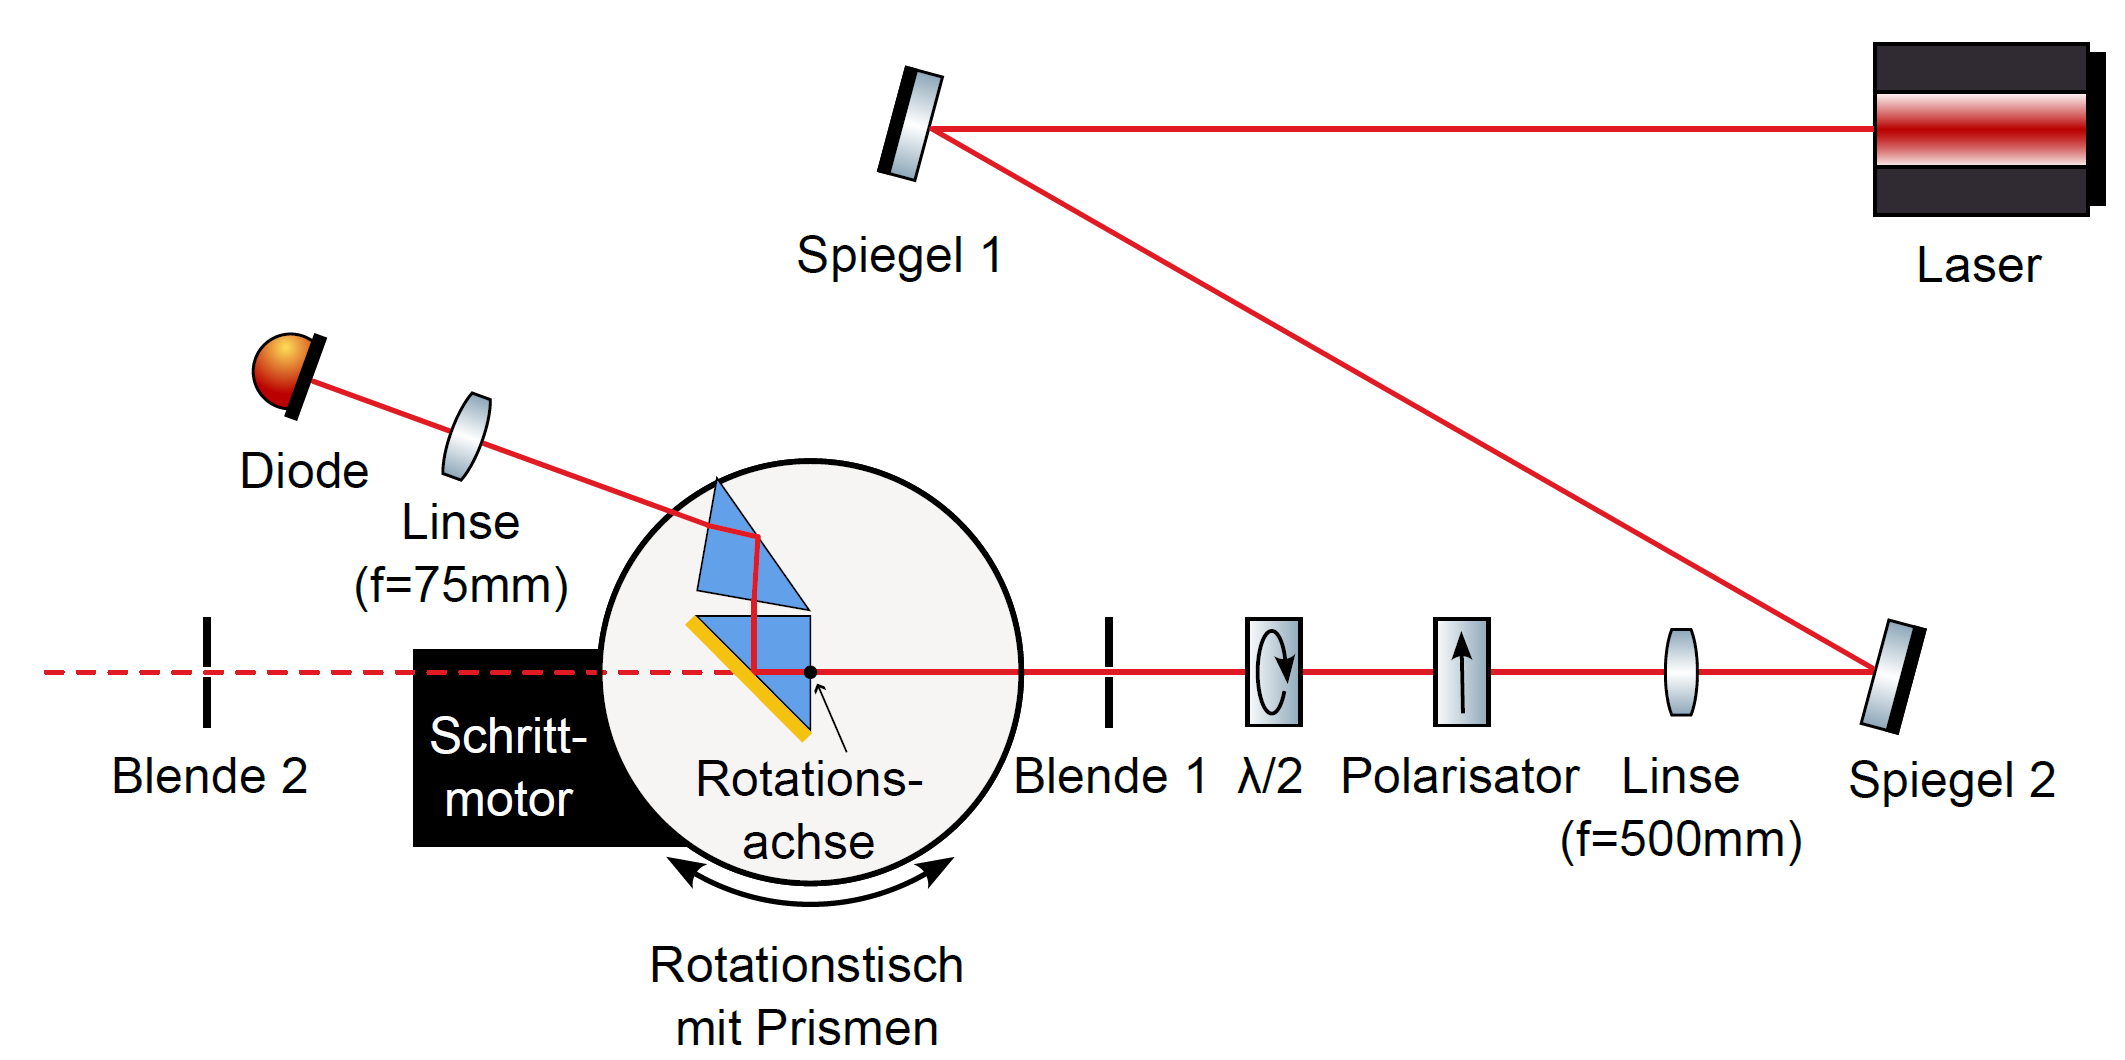
\includegraphics[width=0.6\linewidth]{../figs/versuchsteil1_aufbau.png}
	\caption{Versuchsaufbau des ORS-Experiments mit einem Laser und einer Zwei-Prismen-\\Konfiguration \cite{skript}.}
	\label{fig:versuchsteil1_aufbau}
\end{figure} Dazu wird zunächst der Laserstrahl des monochromatischen Diodenlasers (\SI{785}{\nano \meter} Wellenlänge) mithilfe zweier Spiegel entlang einer Lochreihe
in einer Höhe von etwa \SI{10}{\cm} parallel zum optischen Tisch ausgerichtet. Dazu werden die beiden Spiegel und zwei Iris-Blenden wie in \cref{fig:versuchsteil1_aufbau}
ebenfalls auf eine Höhe von etwa \SI{10}{\cm} eingestellt. Um den Laserstrahl auszurichten, werden iterativ Spiegel 1 bzw. Spiegel 2 justiert, um den Laserstrahl
auf Blende 1 bzw. Blende 2 zu zentrieren. Dieses Justierungsverfahren wird solange durchgeführt, bis beide Blenden nahezu vollständig geschlossen sind und der Laserstrahl
immer noch hinter Blende 2 zu beobachten ist.\par
Um die leichte Divergenz des Diodenlasers zu kompensieren, wird hinter Spiegel 2 eine Linse mit einer Brennweite von $f = \SI{500}{\mm}$ zur Fokussierung
des Strahls aufgebaut. Hierbei muss darauf geachtet werden, dass der Strahl weiterhin auf den beiden Blenden zentriert ist.\par
Anschließend werden hinter der Linse ein Linearpolarisator und eine $\lambda/2$-Wellenplatte montiert. Der verwendete Laserstrahl ist zwar vertikal polarisiert,
dennoch wird ein Linearpolarisator zur Gewährleistung einer möglichst perfekten Polarisation verwendet. Die Polarisationsachse muss vertikal orientiert sein.
Auch die optische Achse der Wellenplatte wird zunächst vertikal orientiert, wobei diese Orientierung während der Versuchsdurchführung variiert wird. Der
verwendete Laserstrahl muss linear polarisiert sein, da bei diesem Versuch die Anregung von SPPs bei s- bzw. p-polarisiertem Licht untersucht wird. Der Wechsel
zwischen s- und p-polarisiertem Licht gelingt mit der $\lambda/2$-Wellenplatte, da sich mit dieser die Polarisationsrichtung drehen lässt. Hier muss darauf geachtet werden,
dass der Strahl nicht durch die Optiken beschnitten wird.\par
Nun wird die motorisierte Rotationsbühne, auf der sich die beiden identischen rechtwinkligen BK7-Prismen befinden, auf den optischen Tisch gesetzt, sodass der
Schrittmotor parallel zur Lochreihe und in Richtung Blende 2 ausgerichtet ist und der Laserstrahl die Rotationsachse schneidet. Die Rotationsachse der Rotationsbühne fällt
mit dem Mittelpunkt einer Seite des Prismas, auf dessen Hypotenuse später die zu untersuchenden Proben befestigt werden, zusammen. Das zweite Prisma dient dazu,
dass bei veränderlichem Einfallswinkel des Laserstrahls auf das erste Prisma der Ausfallswinkel des reflektierten Laserstrahls aus der Sicht des Messgerätes unverändert bleibt,
sodass das später eingebaute Messgerät stationär verbaut werden kann und nicht ständig mitgedreht werden muss. Die Funktionsweise dieser Zwei-Prismen-Konfiguration
ist in \cite{prism} erläutert. Allerdings gibt es durch diese Konfiguration einen leichten Strahlversatz hinter dem zweiten Prisma, welcher aber durch eine Linse
mit einer Brennweite von $f = \SI{75}{\mm}$ korrigiert wird. Außerdem wird der Rotationstisch mit den Knöpfen am Kontroller gedreht, bis die Seitenfläche des mittigen Prismas
in etwa senkrecht zur optischen Achse steht. Es wird der Rückreflex des Lasers beobachtet und der Winkel des Rotationstisches korrigiert, bis der Rückreflex durch
die erste Blende läuft. Damit wird die feste Position des Messgerätes festgelegt, da der Laserstrahl nun das zweite Prisma unter einem Winkel von etwa \SI{20}{\degree}
relativ zur Richtung des einlaufenden Laserstrahls verlässt.\par
Nun kan der Chip der Diode mittig in den Laserstrahl gestellt werden, wobei wie schon zuvor erwähnt eine Sammellinse mit einer Brennweite von $f = \SI{75}{\mm}$ hinter
den Rotationstisch mittig in den Strahl gestellt wird. Die Diode erzeugt bei Bestrahlung mit Licht einen Strom, dessen Stromstärke von der Lichtintensität abhängt.
\subsection{Messung}\label{subsec:teil1_messung}
Zunächst wird eine Referenzmessung mit einem unbeschichteten Deckglas durchgeführt. Dazu wird die Hypotenuse des mittigen Prismas mit einem mit Xylol getränkten
Linsenputztuch gereinigt. Anschließend wird dort das Deckglas mithilfe eines Tropfen Immersionsöl (gleicher Brechungsindex wie das Glas des Prismas, womit es
die Messung nicht beeinflusst) befestigt. Der Rotationstisch wird mit dem Kontroller gedreht, bis die Hypotenuse des mittigen Prismas ungefähr senkrecht über der Lochreihe steht. Dann wird der Drehwinkel des
Rotationstisches korrigiert, bis der direkt reflektierte Strahl durch die Blende läuft. Diese Einstellung des Rotationstisches wird als Startwert für die Winkelmessung
benötigt. Diese Position wird mithilfe des Python-Programms \texttt{ORSScan} als Nullposition gespeichert. Nun kann die Intensität des reflektierten Laserstrahls
als Funktion des Einfallswinkel $I_{\mathrm{ref}}(\theta)$ gemessen werden. Diese Messung wird für einen vertikal (s-polarisiert bzw. TE-polarisiert (elektrisches Feld
parallel zur Grenzfläche)) und einen horizontal (p-polarisiert bzw. TM-polarisiert (magnetisches Feld parallel zur Grenzfläche))
polarisierten Laserstrahl durchgeführt. Der vertikal polarisierte Laserstrahl wird erreicht, indem die $\lambda/2$-Wellenplatte auf \SI{0}{\degree} (optische Achse
vertikal zum optischen Tisch) gestellt wird. Entsprechend wird der horizontal polarisierte Laserstrahl erreicht, indem die $\lambda/2$-Wellenplatte anschließend
um \SI{45}{\degree} gedreht wird. Es wird eine Laserleistung von \SI{23,0}{\watt} eingestellt.\par
In dem Python-Programm \texttt{ORSScan} wird ein Winkelbereich von \SI{40}{\degree} bis \SI{45}{\degree} (\cite{prism} wird entnommen, dass in etwa dieser
Winkelbereich für diesen Versuchsteil relevant sein sollte) eingestellt. Zudem wird eine Winkelauflösung von 200 (200 Messpunkte in dem gewählten Winkelbereich) und
eine Mittelung von 50 (es werden 50 Intensitätswerte pro Winkel gemessen und anschließend gemittelt) eingestellt. Aus der Winkelauflösung und dem gewählten Winkelbereich
(dies resultiert in einer Winkelschrittweite von \SI{0,025}{\degree}) lässt sich für den Einfallswinkel $\theta$ eine Unsicherheit von $\Delta \theta = \SI{0,02}{\degree}$ abschätzen.
Die Unsicherheit der gemessenen Intensität (welche für die Zwecke dieses Versuches in willkürlichen Einheiten (w.E.) gemessen wird) ist wesentlich schwieriger abzuschätzen.
Der Diodenlaser sollte bei einer eingestellten Leistung von \SI{23,0}{\watt} relativ konstant laufen. Außerdem sollte die Unsicherheit relativ klein sein, da pro
Datenpunkt über 50 Intensitätswerte gemittelt wird. Für den gemessenen Intensitätsbereich wird daher eine Unsicherheit von $\Delta I = \SI{0,05}{\we}$ gewählt. Diese
sollte noch groß genug sein, sodass die Schwankungen des Diodenlasers berücksichtigt werden. Die aufgenommenen Messwerte sind in \cref{fig:referenz_own} dargestellt.\par
In einem nächsten Schritt werden die Messungen an den vier zur Verfügung stehenden Goldfilmen durchgeführt. Dafür wird zunächst das unbeschichtete Deckglas
von der Hypotenuse des mittigen Prismas entfernt. Nach einer Reinigung der Hypotenuse dieses Prismas kann einer der Goldfilme mit einem Tropfen des Immersionsöls auf
dem Prisma befestigt werden. Hierbei ist darauf zu achten, dass das Gold selber nicht mit dem Immersionsöl in Kontakt kommt. Anschließend kann die Intensität des am
Goldfilm reflektierten Laserstrahls als Funktion des Einfallswinkels $I_{\mathrm{Au}}(\theta)$ sowohl für TM- als auch TE-Polarisation für alle vier Goldfilme gemessen werden. Die Unsicherheiten
werden wie bei der Referenzmessung abgeschätzt/gewählt. Die Rohdaten sind in \cref{fig:gold_own} dargestellt.\par
Es wurde sofort erkannt, dass diese Messergebnisse nicht sinnvoll sind,
da für jeden Goldfilm bei TM-Polarisation ein deutlich erkennbares Minimum zu erwarten ist (der Grund dafür wird später in der Auswertung erläutert). Dies ist lediglich
bei dem vierten Goldfilm der Fall. Doch auch hier sind die Messergebnisse nicht sinnvoll auswertbar, da bei diesem Goldfilm das Ergebnis davon abhängig war, wie der
rechteckige Goldfilm relativ zu der Horizontalen des Optiktisches gedreht wurde. Ein Austausch mit dem Assistenten resultierte in der Erkenntnis, dass die Goldfilme zu
verschmutzt/veraltet sind, um sie für diesen Versuch zu verwenden, weshalb die aufgenommenen Messwerte leider nicht sinnvoll auszuwerten sind. Dennoch sind die Rohdaten
aus Gründen der Vollständigkeit in \url{https://uni-bonn.sciebo.de/s/5WDpU2gFKodo5WJ} hinterlegt. Nach Rücksprache mit dem Assistenten werden für diesen Versuchsteil auswertbare Daten, die nicht von den
Experimentierenden aufgenommen wurden, zur Verfügung gestellt. Diese werden aus Gründen des Urheberrechtes nicht verlinkt (dies ist auch nicht notwendig, da
der Assistent selber über diese Daten verfügt). Offensichtlich müssen auch die selbst aufgenommenen Daten der Referenzmessung verworfen werden, da zu den vom Assistenten
bereitgestellten Daten zu den Goldproben-Messungen die zugehörige Referenzmessung verwendet werden muss. Diese vom Assistenten bereitgestellten Rohdaten sind im \hyperref[sec:anhang]{Anhang} in \cref{fig:referenz} und \cref{fig:gold} dargestellt.
Die Winkelunsicherheiten werden wie bei den selbst aufgenommenen Messwerten gewählt, da der ausgewählte Winkelbereich und die Winkelauflösung identisch sind. Die Intensitätsunsicherheiten
werden nun abgeschätzt, indem ausgenutzt wird dass bei der Referenzmessung oberhalb eines Grenzwinkels aufgrund von Totalreflexion eine konstante reflektierte Intensität und
bei den Messungen zu den Goldfilmen bei TE-Polarisation (da hier keine OPPs angeregt werden) eine konstante reflektierte Intensität erwartet wird. So wird durch die Ausreißer nach oben und nach unten eine
Unsicherheit von $\Delta I = \SI{0,025}{\we}$ festgelegt.
\begin{figure}[H]
	\centering
	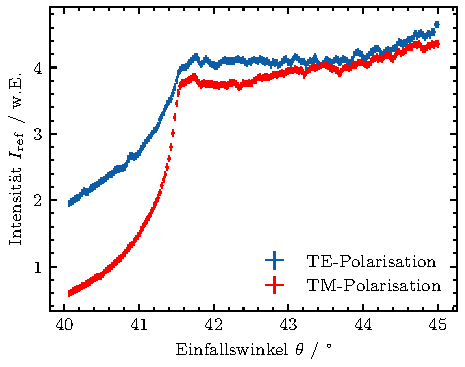
\includegraphics[width=0.4\linewidth]{../figs/referenz_own.pdf}
	\caption{Rohdaten der Referenzmessung für ein unbeschichtetes Deckglas für TM- und TE-Polarisation (die Winkelunsicherheiten sind für diesen Winkelbereich zu klein, um erkennbar zu sein).}
	\label{fig:referenz_own}
\end{figure}
\begin{figure}[H]
    \centering
    \begin{subfigure}{0.4\textwidth}
        \centering
        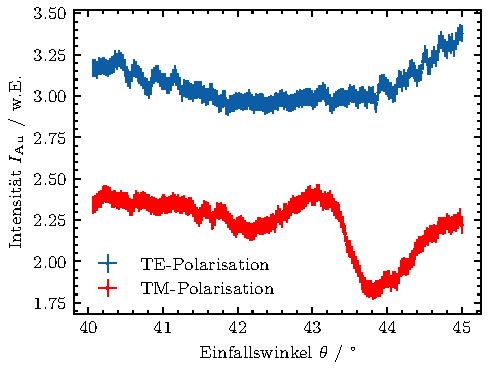
\includegraphics[width=\linewidth]{../figs/au1_own}
        \caption{Goldfilm 1}
    \end{subfigure}
    \begin{subfigure}{0.4\textwidth}
        \centering
        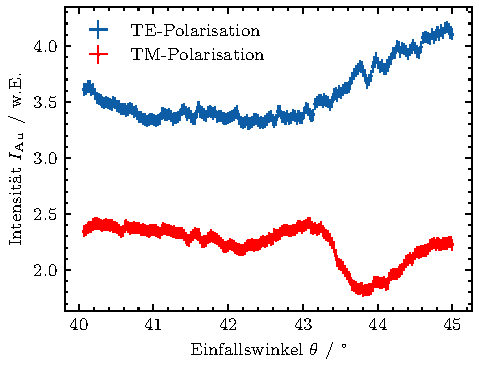
\includegraphics[width=\linewidth]{../figs/au2_own}
        \caption{Goldfilm 2}
    \end{subfigure}
    \begin{subfigure}{0.4\textwidth}
        \centering
        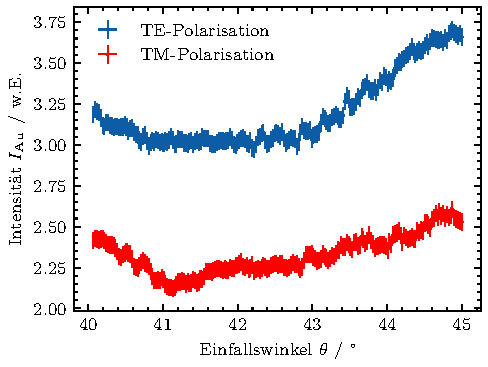
\includegraphics[width=\linewidth]{../figs/au3_own}
        \caption{Goldfilm 3}
    \end{subfigure}
    \begin{subfigure}{0.4\textwidth}
        \centering
        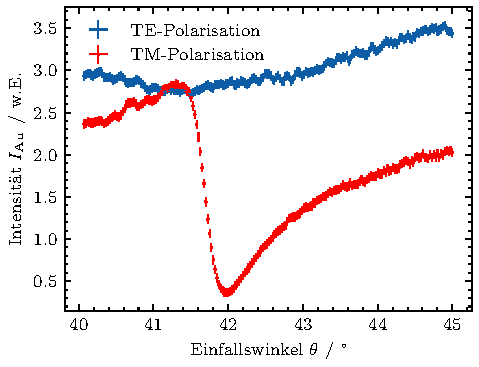
\includegraphics[width=\linewidth]{../figs/au4_own}
        \caption{Goldfilm 4}
    \end{subfigure}
    \caption{Rohdaten der Reflexionsmessungen an vier Goldfilmen für TM- und TE-Polarisation (die Winkelunsicherheiten sind für diesen Winkelbereich zu klein, um erkennbar zu sein).}\label{fig:gold_own}
\end{figure}\newpage
\subsection{Auswertung}\label{subsec:teil1_auswertung}
\subsubsection*{Bestimmung des Brechungsindex $n_{\mathrm{Prisma}}$ der Prismen mithilfe der Referenzmessung}\label{subsubsec:referenz}
Zuerst wird mithilfe der Referenzmessung $I_{\mathrm{ref}}(\theta)$ der Brechungsindex $n_{\mathrm{Prisma}}$ der Prismen bei der Laser-Wellenlänge \SI{785}{\nm}
bestimmt. Zunächst lässt sich leicht zeigen, dass bei der Bestimmung von $n_{\mathrm{Prisma}}$ der Brechungsindex des Immersionsöls und des Deckglases keine Rolle spielen,
indem das Brechungsgesetz verwendet wird. Dieses lautet für die Lichtbrechung an der Grenzfläche zwischen zwei Medien
\begin{equation*}
    n_1 \sin(\theta_{\mathrm{i}}) = n_2 \sin(\theta_{\mathrm{t}}),
\end{equation*} wobei $n_1$ und $n_2$ die Brechungsindizes der beiden Medien und $\theta_{\mathrm{i}}$ bzw. $\theta_{\mathrm{t}}$ der Ein- bzw. Ausfallswinkel des Lichtes
ist (siehe \cite{linden_optik}). Bei der Referenzmessung ist der Laser zunächst auf das Prisma, dann auf den Ölfilm, anschließend auf das Deckglas und schließlich auf die Luft
gefallen. Damit folgt durch Anwenden des Brechungsgesetzes:
\begin{align*}
    n_{\mathrm{Prisma}} \sin(\theta) &= n_{\mathrm{Öl}} \sin(\theta_1) \\
    n_{\mathrm{Öl}} \sin(\theta_1) &= n_{\mathrm{Glas}} \sin(\theta_2) \\
    n_{\mathrm{Glas}} \sin(\theta_2) &= n_{\mathrm{Luft}} \sin(\theta_3) .
\end{align*} Durch Ausnutzen der Gleichungskette folgt insgesamt
\begin{equation*}
    n_{\mathrm{Prisma}} \sin(\theta) = n_{\mathrm{Luft}} \sin(\theta_3) .
\end{equation*} Dies beschreibt nun die Brechung an einer Grenzfläche zwischen Prisma und Luft mit dem Einfallswinkel $\theta$ und dem Ausfallswinkel $\theta_3$, womit
zur Bestimmung von $n_{\mathrm{Prisma}}$ der Brechungsindex des Öls und des Deckglases keine Rolle spielen. Damit kann bei der Bestimmung von $n_{\mathrm{Prisma}}$
so vorgegangen werden, als ob das Licht an einer Grenzfläche zwischen Prisma und Luft (nur zwei Medien) gebrochen wird.\par
Zur Bestimmung von $n_{\mathrm{Prisma}}$ wird der Reflexionsgrad benötigt, welcher den Anteil der reflektierten Intensität relativ zur einfallenden Intensität beschreibt.
Für TM-Polarisation berechnet sich der Reflexionsgrad durch $R_{\mathrm{TM}} = |r_{\mathrm{TM}}|^2$ und für TE-Polarisation durch $R_{\mathrm{TE}} = |r_{\mathrm{TE}}|^2$.
Hierbei sind die Reflexionskoeffizienten nach \cite{linden_optik} und durch Anwenden des Brechungsgesetzes durch
\begin{equation}
    r_{\mathrm{TM}} = \frac{n_{\mathrm{Luft}}\cos(\theta) - n_{\mathrm{Prisma}}\sqrt{1 - \left(\frac{n_{\mathrm{Prisma}}}{n_{\mathrm{Luft}}}\sin(\theta)\right)^2}}{n_{\mathrm{Prisma}}\sqrt{1 - \left(\frac{n_{\mathrm{Prisma}}}{n_{\mathrm{Luft}}}\sin(\theta)\right)^2} + n_{\mathrm{Luft}}\cos(\theta)}
\end{equation} bzw.
\begin{equation}
    r_{\mathrm{TE}} = \frac{n_{\mathrm{Prisma}}\cos(\theta) - n_{\mathrm{Luft}}\sqrt{1 - \left(\frac{n_{\mathrm{Prisma}}}{n_{\mathrm{Luft}}}\sin(\theta)\right)^2}}{n_{\mathrm{Prisma}}\cos(\theta) + n_{\mathrm{Luft}}\sqrt{1 - \left(\frac{n_{\mathrm{Prisma}}}{n_{\mathrm{Luft}}}\sin(\theta)\right)^2}}
\end{equation} gegeben. Damit folgt also für die Reflexionsgrade
\begin{equation}\label{eq:reflexionsgrad_tm}
    R_{\mathrm{TM}} = \abs{\frac{n_{\mathrm{Prisma}}\sqrt{1 - \left(\frac{n_{\mathrm{Prisma}}}{n_{\mathrm{Luft}}}\sin(\theta)\right)^2} - n_{\mathrm{Luft}}\cos(\theta)}{n_{\mathrm{Prisma}}\sqrt{1 - \left(\frac{n_{\mathrm{Prisma}}}{n_{\mathrm{Luft}}}\sin(\theta)\right)^2} + n_{\mathrm{Luft}}\cos(\theta)}}^2
\end{equation} bzw.
\begin{equation}\label{eq:reflexionsgrad_te}
    R_{\mathrm{TE}} = \abs{\frac{n_{\mathrm{Prisma}}\cos(\theta) - n_{\mathrm{Luft}}\sqrt{1 - \left(\frac{n_{\mathrm{Prisma}}}{n_{\mathrm{Luft}}}\sin(\theta)\right)^2}}{n_{\mathrm{Prisma}}\cos(\theta) + n_{\mathrm{Luft}}\sqrt{1 - \left(\frac{n_{\mathrm{Prisma}}}{n_{\mathrm{Luft}}}\sin(\theta)\right)^2}}}^2 .
\end{equation} Die gemessenen Werte für $R_{\mathrm{TM}}$ bzw. $R_{\mathrm{TE}}$ ergeben sich mithilfe der Intensitätsmessungen zu
\begin{equation}\label{eq:reflexionsgrad_gemessen}
    R_{\mathrm{TM/TE}} = \frac{I_{\mathrm{ref}}(\theta)}{I_{\mathrm{ref,max}}} ,
\end{equation} wobei die Unsicherheiten durch
\begin{equation*}
    \Delta R_{\mathrm{TM/TE}} = \sqrt{\left(\frac{\Delta I_{\mathrm{ref}}(\theta)}{I_{\mathrm{ref,max}}}\right)^2 + \left(\frac{I_{\mathrm{ref}}(\theta)}{I_{\mathrm{ref,max}}^2}\Delta I_{\mathrm{ref,max}}\right)^2}
\end{equation*} gegeben sind. Die Unsicherheiten für $I_{\mathrm{ref}}$ und $I_{\mathrm{ref,max}}$ sind (wie in \cref{subsec:teil1_messung} beschrieben) zu \SI{0.025}{\we} gewählt.
Der maximale Wert der Intensitätsmessung wird leicht aus dem aufgenommenen Datensatz mithilfe des Python-Moduls \texttt{numpy} extrahiert. \cref{eq:reflexionsgrad_gemessen}
ist gültig, da die reflektierte Intensität bei Totalreflexion maximal wird und dann (näherungsweise) der einlaufenden Intensität entspricht.\par
Für die folgende Anpassung (und alle weiteren Anpassungen, die in dieser Auswertung durchgeführt werden) wird aus dem Python-Modul \texttt{scipy} die Funktion
\texttt{Orthogonal Distance Regression} (\texttt{ODR}) verwendet. Bei diesem Verfahren wird die Güte der Anpassung durch die \textit{Residual Variance} $\chi_{\mathrm{res}}^2$
beschrieben. Als Anpassungsfunktionen werden \cref{eq:reflexionsgrad_tm} und \cref{eq:reflexionsgrad_te} verwendet. Für den Brechungsindex von Luft wird
$n_{\mathrm{Luft}} = 1.000292$ \cite{wiki:brechungsindex} genommen. Die Winkelunsicherheiten sind wie in \cref{subsec:teil1_messung} zu $\Delta \theta = \SI{0,02}{\degree}$
gewählt. Die Ergebnisse der Anpassung sind in \cref{fig:glas_fit} dargestellt. Für die Anpassung ist nur der Winkelbereich bis zu dem Winkel relevant, ab dem Totalreflexion auftritt und der
Reflexionsgrad $R \approx 1$ ist.
\begin{figure}[H]
    \centering
    \begin{subfigure}{0.45\textwidth}
        \centering
        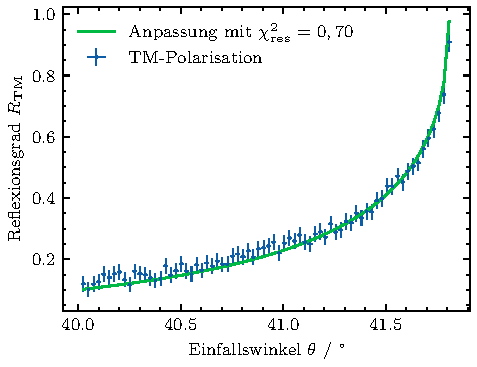
\includegraphics[width=\linewidth]{../figs/glas_ppol_fit}
        \caption{TM-Polarisation}
    \end{subfigure}
    \begin{subfigure}{0.45\textwidth}
        \centering
        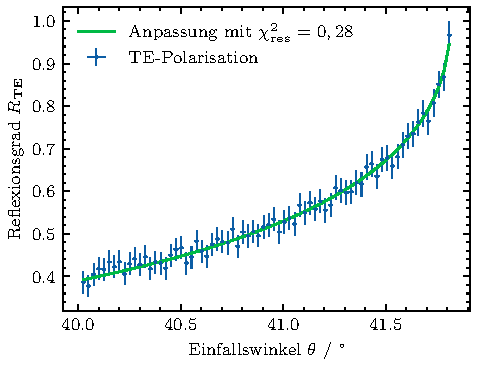
\includegraphics[width=\linewidth]{../figs/glas_spol_fit}
        \caption{TE-Polarisation}
    \end{subfigure}
    \caption{Anpassung der theoretischen Formeln für die Reflexionsgrade $R_{\mathrm{TM}}$ und $R_{\mathrm{TE}}$ an die Messwerte der Referenzmessung
    zur Bestimmung des Brechungsindex $n_{\mathrm{Prisma}}$.}\label{fig:glas_fit}
\end{figure} Anhand der angegebenen Werte für die Güte ist zu erkennen, dass eine Überanpassung erreicht wurde, was eventuell durch die gewählten Unsicherheiten
zu begründen ist.